% !TEX root = main.tex

% June 14, Part 3

\section*{Implementation of new interpolation scheme}
We were not able to successfully compute the approximate Radon transform via bi-linear interpolation or Shepard's method.
Dr. Rossmanith showed us an alternative interpolation method.
\par 
We discretize the unit disk by discretizing the interval $[0, \pi]$ into $N_{\omega}$ many points, with a spacing of $\delta \omega$ between each point.
Along each angle $\omega_{i}$, we draw a line that goes through the origin of disk, and we discretize that line using $N_{s}$ many Chebyshev points.
For $N_{\omega} = 50$ and $N_{s} = 50$, the grid looks like the following
\begin{figure}[H]
	\centering
	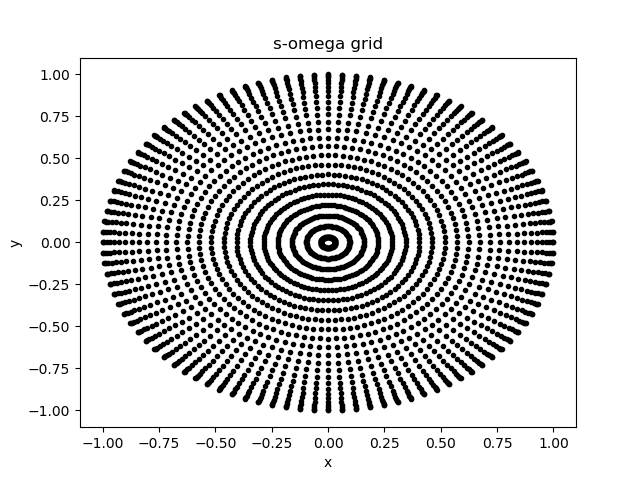
\includegraphics[width=0.75\textwidth]{s_omega_grid.png}
\end{figure}
We programmed the new interpolation scheme in \verb|radon_transfom_v5.py| within the function \verb|radon(f_vec, Ns, Nw, Nq)|, where the argument \verb|f_vec| is a $N_{\omega} \times N_s$ by $1$ long vector, \verb|Ns| is equal to $N_{s}$ i.e. the number of discretization points in the $s$-direction, \verb|Nw| is equal to $N_{\omega}$ i.e. the number of angles in the angular discretization, and \verb|Nq| is equal to the number of quadrature points we use to approximate the line integral at every mesh point.
\par
We originally define \verb|f_vec| to be a $N_{\omega} \times N_{s}$ matrix whose entries are $f$ (the function whose Radon transform we are taking) evaluated at all the points in $s$-$\omega$ discretization. 
We then flatten \verb|f_vec| to be a vector with $N_{\omega} \times N_{s}$ entries.
To convert between the position of a doubly indexed point in the mesh (for example, the point given by $(s_{j}, \omega_{i})$), we use the following linear index
\begin{align*}
	p & = i \times N_{s} + j
\end{align*}
The reason why we write \verb|f_vec| in this manner is because we eventually want to write the Radon transform of \verb|f_vec| as a matrix-vector multiplication.
\par
We obtain \verb|Ns| Chebyshev points and \verb|Nw| equispaced angles on the interval $[0, \pi]$, and we also compute \verb|Nq| many 